\documentclass{standalone}
\usepackage{tikz}
\usetikzlibrary{patterns, positioning}


\begin{document}
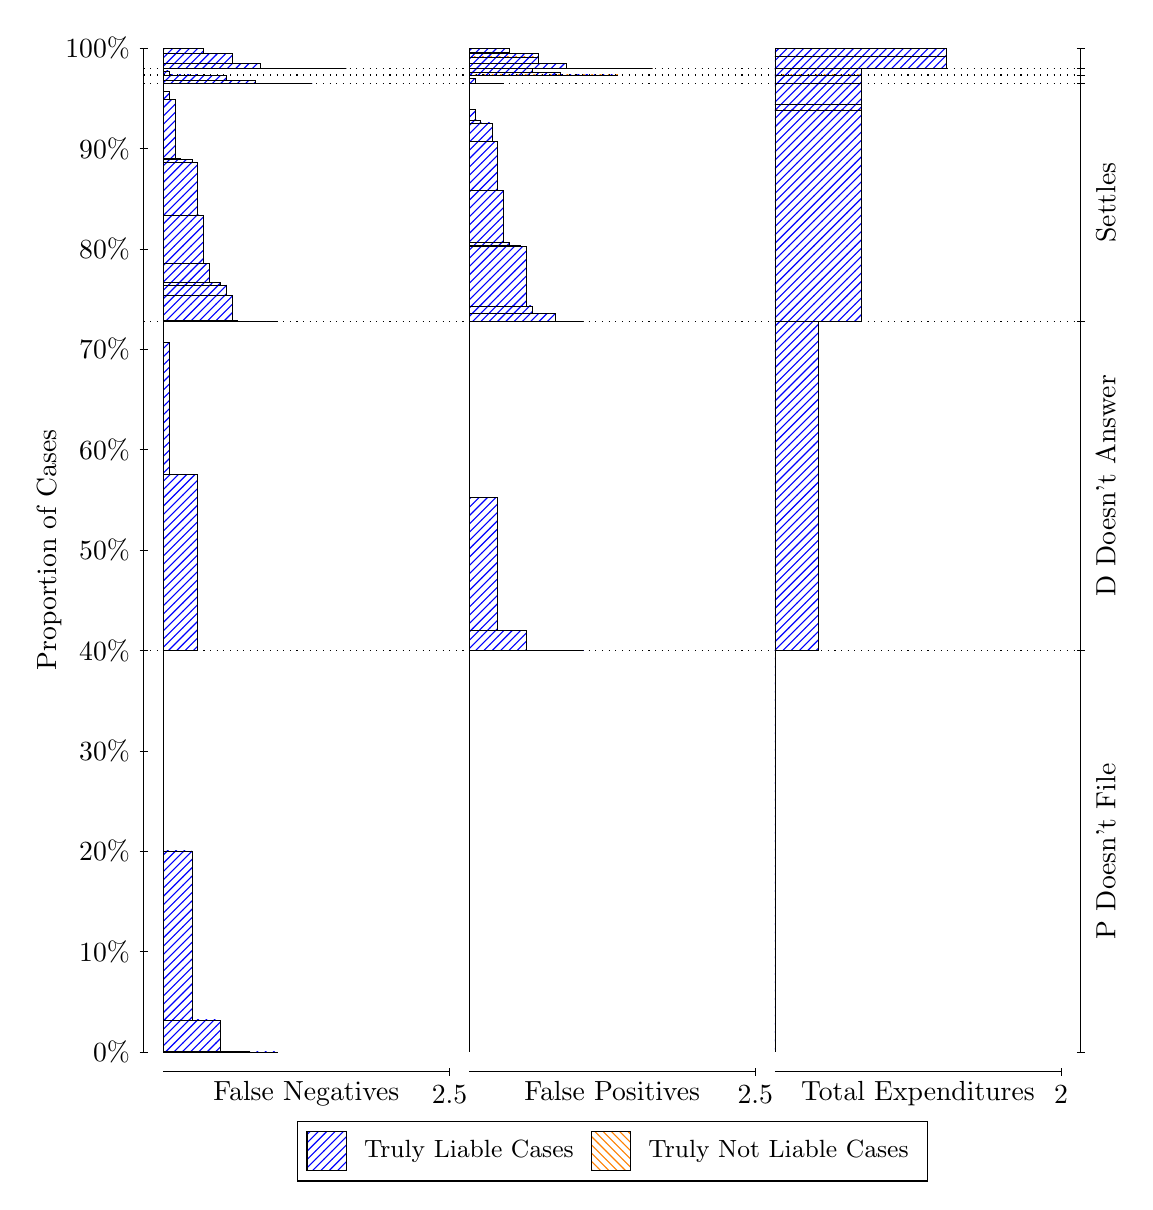
\begin{tikzpicture}
\draw[black, very thin] (1.5,1.75) -- (1.5,14.5);
\node[rotate=90, text=black, anchor=center] at (0.3, 8.125) {Proportion of Cases};
\draw[black, very thin] (1.45,1.75) -- (1.55,1.75);
\node[text=black, anchor=east] at (1.45, 1.75) {0\%};
\draw[black, very thin] (1.45,3.025) -- (1.55,3.025);
\node[text=black, anchor=east] at (1.45, 3.025) {10\%};
\draw[black, very thin] (1.45,4.3) -- (1.55,4.3);
\node[text=black, anchor=east] at (1.45, 4.3) {20\%};
\draw[black, very thin] (1.45,5.575) -- (1.55,5.575);
\node[text=black, anchor=east] at (1.45, 5.575) {30\%};
\draw[black, very thin] (1.45,6.85) -- (1.55,6.85);
\node[text=black, anchor=east] at (1.45, 6.85) {40\%};
\draw[black, very thin] (1.45,8.125) -- (1.55,8.125);
\node[text=black, anchor=east] at (1.45, 8.125) {50\%};
\draw[black, very thin] (1.45,9.4) -- (1.55,9.4);
\node[text=black, anchor=east] at (1.45, 9.4) {60\%};
\draw[black, very thin] (1.45,10.675) -- (1.55,10.675);
\node[text=black, anchor=east] at (1.45, 10.675) {70\%};
\draw[black, very thin] (1.45,11.95) -- (1.55,11.95);
\node[text=black, anchor=east] at (1.45, 11.95) {80\%};
\draw[black, very thin] (1.45,13.225) -- (1.55,13.225);
\node[text=black, anchor=east] at (1.45, 13.225) {90\%};
\draw[black, very thin] (1.45,14.5) -- (1.55,14.5);
\node[text=black, anchor=east] at (1.45, 14.5) {100\%};

\draw[black, very thin] (13.4,1.75) -- (13.4,14.5);
\draw[black, very thin] (13.35,1.75) -- (13.45,1.75);
\node[anchor=west] at (13.35, 1.75) {};
\draw[black, very thin] (13.35,6.8489) -- (13.45,6.8489);
\node[anchor=west] at (13.35, 6.8489) {};
\draw[black, very thin] (13.35,11.028) -- (13.45,11.028);
\node[anchor=west] at (13.35, 11.028) {};
\draw[black, very thin] (13.35,14.049) -- (13.45,14.049);
\node[anchor=west] at (13.35, 14.049) {};
\draw[black, very thin] (13.35,14.158) -- (13.45,14.158);
\node[anchor=west] at (13.35, 14.158) {};
\draw[black, very thin] (13.35,14.239) -- (13.45,14.239);
\node[anchor=west] at (13.35, 14.239) {};
\draw[black, very thin] (13.35,14.5) -- (13.45,14.5);
\node[anchor=west] at (13.35, 14.5) {};

\draw[black, very thin, pattern color=blue, pattern=north east lines] (1.75,1.75) rectangle (3.2033,1.75);
\draw[black, very thin, pattern color=blue, pattern=north east lines] (1.75,1.75) rectangle (2.84,1.7534);
\draw[black, very thin, pattern color=blue, pattern=north east lines] (1.75,1.7534) rectangle (2.4767,2.158);
\draw[black, very thin, pattern color=blue, pattern=north east lines] (1.75,2.158) rectangle (2.1133,4.3029);
\draw[black, very thin, pattern color=orange, pattern=north west lines] (1.75,4.3029) rectangle (1.75,4.3029);
\draw[black, very thin, pattern color=blue, pattern=north east lines] (1.75,4.3029) rectangle (1.75,6.8489);
\draw[black, very thin, pattern color=blue, pattern=north east lines] (1.75,6.8489) rectangle (2.186,9.0805);
\draw[black, very thin, pattern color=blue, pattern=north east lines] (1.75,9.0805) rectangle (1.8227,10.768);
\draw[black, very thin, pattern color=orange, pattern=north west lines] (1.75,10.768) rectangle (1.75,10.768);
\draw[black, very thin, pattern color=blue, pattern=north east lines] (1.75,10.768) rectangle (1.75,11.028);
\draw[black, very thin, pattern color=blue, pattern=north east lines] (1.75,11.028) rectangle (3.2033,11.028);
\draw[black, very thin, pattern color=blue, pattern=north east lines] (1.75,11.028) rectangle (3.058,11.028);
\draw[black, very thin, pattern color=blue, pattern=north east lines] (1.75,11.028) rectangle (2.9127,11.028);
\draw[black, very thin, pattern color=blue, pattern=north east lines] (1.75,11.028) rectangle (2.84,11.028);
\draw[black, very thin, pattern color=blue, pattern=north east lines] (1.75,11.028) rectangle (2.6947,11.041);
\draw[black, very thin, pattern color=blue, pattern=north east lines] (1.75,11.041) rectangle (2.622,11.357);
\draw[black, very thin, pattern color=blue, pattern=north east lines] (1.75,11.357) rectangle (2.5493,11.491);
\draw[black, very thin, pattern color=blue, pattern=north east lines] (1.75,11.491) rectangle (2.4767,11.527);
\draw[black, very thin, pattern color=blue, pattern=north east lines] (1.75,11.527) rectangle (2.3313,11.765);
\draw[black, very thin, pattern color=blue, pattern=north east lines] (1.75,11.765) rectangle (2.2587,12.381);
\draw[black, very thin, pattern color=blue, pattern=north east lines] (1.75,12.381) rectangle (2.186,13.047);
\draw[black, very thin, pattern color=blue, pattern=north east lines] (1.75,13.047) rectangle (2.1133,13.083);
\draw[black, very thin, pattern color=blue, pattern=north east lines] (1.75,13.083) rectangle (1.968,13.096);
\draw[black, very thin, pattern color=blue, pattern=north east lines] (1.75,13.096) rectangle (1.8953,13.852);
\draw[black, very thin, pattern color=blue, pattern=north east lines] (1.75,13.852) rectangle (1.8227,13.95);
\draw[black, very thin, pattern color=orange, pattern=north west lines] (1.75,13.95) rectangle (1.75,13.95);
\draw[black, very thin, pattern color=blue, pattern=north east lines] (1.75,13.95) rectangle (1.75,14.049);
\draw[black, very thin, pattern color=blue, pattern=north east lines] (1.75,14.049) rectangle (3.6393,14.049);
\draw[black, very thin, pattern color=blue, pattern=north east lines] (1.75,14.049) rectangle (3.276,14.049);
\draw[black, very thin, pattern color=blue, pattern=north east lines] (1.75,14.049) rectangle (2.9127,14.09);
\draw[black, very thin, pattern color=blue, pattern=north east lines] (1.75,14.09) rectangle (2.5493,14.156);
\draw[black, very thin, pattern color=blue, pattern=north east lines] (1.75,14.156) rectangle (2.186,14.158);
\draw[black, very thin, pattern color=orange, pattern=north west lines] (1.75,14.158) rectangle (1.75,14.158);
\draw[black, very thin, pattern color=blue, pattern=north east lines] (1.75,14.158) rectangle (2.186,14.159);
\draw[black, very thin, pattern color=blue, pattern=north east lines] (1.75,14.159) rectangle (1.8227,14.209);
\draw[black, very thin, pattern color=orange, pattern=north west lines] (1.75,14.209) rectangle (1.75,14.209);
\draw[black, very thin, pattern color=blue, pattern=north east lines] (1.75,14.209) rectangle (1.75,14.239);
\draw[black, very thin, pattern color=blue, pattern=north east lines] (1.75,14.239) rectangle (4.0753,14.239);
\draw[black, very thin, pattern color=blue, pattern=north east lines] (1.75,14.239) rectangle (3.712,14.239);
\draw[black, very thin, pattern color=blue, pattern=north east lines] (1.75,14.239) rectangle (3.3487,14.243);
\draw[black, very thin, pattern color=blue, pattern=north east lines] (1.75,14.243) rectangle (2.9853,14.303);
\draw[black, very thin, pattern color=blue, pattern=north east lines] (1.75,14.303) rectangle (2.622,14.435);
\draw[black, very thin, pattern color=blue, pattern=north east lines] (1.75,14.435) rectangle (2.2587,14.495);
\draw[black, very thin, pattern color=blue, pattern=north east lines] (1.75,14.495) rectangle (1.8953,14.5);
\draw[black, very thin, pattern color=orange, pattern=north west lines] (1.75,14.5) rectangle (1.75,14.5);
\draw[black, very thin, pattern color=blue, pattern=north east lines] (1.75,14.5) rectangle (1.75,14.5);
\draw[black, very thin, pattern color=orange, pattern=north west lines] (5.6333,1.75) rectangle (5.6333,1.75);
\draw[black, very thin, pattern color=blue, pattern=north east lines] (5.6333,1.75) rectangle (5.6333,6.8489);
\draw[black, very thin, pattern color=orange, pattern=north west lines] (5.6333,6.8489) rectangle (7.0867,6.8489);
\draw[black, very thin, pattern color=blue, pattern=north east lines] (5.6333,6.8489) rectangle (7.0867,6.8489);
\draw[black, very thin, pattern color=blue, pattern=north east lines] (5.6333,6.8489) rectangle (6.7233,6.8493);
\draw[black, very thin, pattern color=blue, pattern=north east lines] (5.6333,6.8493) rectangle (6.36,7.1088);
\draw[black, very thin, pattern color=blue, pattern=north east lines] (5.6333,7.1088) rectangle (5.9967,8.7962);
\draw[black, very thin, pattern color=blue, pattern=north east lines] (5.6333,8.7962) rectangle (5.6333,11.028);
\draw[black, very thin, pattern color=orange, pattern=north west lines] (5.6333,11.028) rectangle (7.0867,11.028);
\draw[black, very thin, pattern color=blue, pattern=north east lines] (5.6333,11.028) rectangle (7.0867,11.028);
\draw[black, very thin, pattern color=orange, pattern=north west lines] (5.6333,11.028) rectangle (6.796,11.028);
\draw[black, very thin, pattern color=blue, pattern=north east lines] (5.6333,11.028) rectangle (6.796,11.028);
\draw[black, very thin, pattern color=blue, pattern=north east lines] (5.6333,11.028) rectangle (6.7233,11.127);
\draw[black, very thin, pattern color=orange, pattern=north west lines] (5.6333,11.127) rectangle (6.6507,11.127);
\draw[black, very thin, pattern color=blue, pattern=north east lines] (5.6333,11.127) rectangle (6.6507,11.127);
\draw[black, very thin, pattern color=orange, pattern=north west lines] (5.6333,11.127) rectangle (6.5053,11.127);
\draw[black, very thin, pattern color=blue, pattern=north east lines] (5.6333,11.127) rectangle (6.5053,11.127);
\draw[black, very thin, pattern color=blue, pattern=north east lines] (5.6333,11.127) rectangle (6.4327,11.225);
\draw[black, very thin, pattern color=blue, pattern=north east lines] (5.6333,11.225) rectangle (6.36,11.981);
\draw[black, very thin, pattern color=blue, pattern=north east lines] (5.6333,11.981) rectangle (6.2873,11.993);
\draw[black, very thin, pattern color=blue, pattern=north east lines] (5.6333,11.993) rectangle (6.142,12.03);
\draw[black, very thin, pattern color=blue, pattern=north east lines] (5.6333,12.03) rectangle (6.0693,12.696);
\draw[black, very thin, pattern color=blue, pattern=north east lines] (5.6333,12.696) rectangle (5.9967,13.312);
\draw[black, very thin, pattern color=blue, pattern=north east lines] (5.6333,13.312) rectangle (5.924,13.55);
\draw[black, very thin, pattern color=blue, pattern=north east lines] (5.6333,13.55) rectangle (5.7787,13.586);
\draw[black, very thin, pattern color=blue, pattern=north east lines] (5.6333,13.586) rectangle (5.706,13.72);
\draw[black, very thin, pattern color=blue, pattern=north east lines] (5.6333,13.72) rectangle (5.6333,14.049);
\draw[black, very thin, pattern color=orange, pattern=north west lines] (5.6333,14.049) rectangle (6.0693,14.049);
\draw[black, very thin, pattern color=blue, pattern=north east lines] (5.6333,14.049) rectangle (6.0693,14.05);
\draw[black, very thin, pattern color=blue, pattern=north east lines] (5.6333,14.05) rectangle (5.706,14.117);
\draw[black, very thin, pattern color=blue, pattern=north east lines] (5.6333,14.117) rectangle (5.6333,14.158);
\draw[black, very thin, pattern color=orange, pattern=north west lines] (5.6333,14.158) rectangle (7.5227,14.158);
\draw[black, very thin, pattern color=blue, pattern=north east lines] (5.6333,14.158) rectangle (7.5227,14.158);
\draw[black, very thin, pattern color=blue, pattern=north east lines] (5.6333,14.158) rectangle (7.1593,14.158);
\draw[black, very thin, pattern color=blue, pattern=north east lines] (5.6333,14.158) rectangle (6.796,14.188);
\draw[black, very thin, pattern color=blue, pattern=north east lines] (5.6333,14.188) rectangle (6.4327,14.238);
\draw[black, very thin, pattern color=blue, pattern=north east lines] (5.6333,14.238) rectangle (6.0693,14.239);
\draw[black, very thin, pattern color=orange, pattern=north west lines] (5.6333,14.239) rectangle (7.9587,14.239);
\draw[black, very thin, pattern color=blue, pattern=north east lines] (5.6333,14.239) rectangle (7.9587,14.239);
\draw[black, very thin, pattern color=orange, pattern=north west lines] (5.6333,14.239) rectangle (7.5953,14.239);
\draw[black, very thin, pattern color=blue, pattern=north east lines] (5.6333,14.239) rectangle (7.5953,14.239);
\draw[black, very thin, pattern color=orange, pattern=north west lines] (5.6333,14.239) rectangle (7.232,14.239);
\draw[black, very thin, pattern color=blue, pattern=north east lines] (5.6333,14.239) rectangle (7.232,14.244);
\draw[black, very thin, pattern color=blue, pattern=north east lines] (5.6333,14.244) rectangle (6.8687,14.304);
\draw[black, very thin, pattern color=orange, pattern=north west lines] (5.6333,14.304) rectangle (6.8687,14.304);
\draw[black, very thin, pattern color=blue, pattern=north east lines] (5.6333,14.304) rectangle (6.8687,14.305);
\draw[black, very thin, pattern color=blue, pattern=north east lines] (5.6333,14.305) rectangle (6.5053,14.388);
\draw[black, very thin, pattern color=orange, pattern=north west lines] (5.6333,14.388) rectangle (6.5053,14.388);
\draw[black, very thin, pattern color=blue, pattern=north east lines] (5.6333,14.388) rectangle (6.5053,14.436);
\draw[black, very thin, pattern color=blue, pattern=north east lines] (5.6333,14.436) rectangle (6.142,14.447);
\draw[black, very thin, pattern color=blue, pattern=north east lines] (5.6333,14.447) rectangle (6.142,14.496);
\draw[black, very thin, pattern color=blue, pattern=north east lines] (5.6333,14.496) rectangle (5.7787,14.496);
\draw[black, very thin, pattern color=blue, pattern=north east lines] (5.6333,14.496) rectangle (5.7787,14.5);
\draw[black, very thin, pattern color=blue, pattern=north east lines] (5.6333,14.5) rectangle (5.6333,14.5);
\draw[black, very thin, pattern color=orange, pattern=north west lines] (9.5167,1.75) rectangle (9.5167,1.75);
\draw[black, very thin, pattern color=blue, pattern=north east lines] (9.5167,1.75) rectangle (9.5167,6.8489);
\draw[black, very thin, pattern color=orange, pattern=north west lines] (9.5167,6.8489) rectangle (10.062,6.8489);
\draw[black, very thin, pattern color=blue, pattern=north east lines] (9.5167,6.8489) rectangle (10.062,11.028);
\draw[black, very thin, pattern color=orange, pattern=north west lines] (9.5167,11.028) rectangle (10.607,11.028);
\draw[black, very thin, pattern color=blue, pattern=north east lines] (9.5167,11.028) rectangle (10.607,13.713);
\draw[black, very thin, pattern color=orange, pattern=north west lines] (9.5167,13.713) rectangle (10.607,13.713);
\draw[black, very thin, pattern color=blue, pattern=north east lines] (9.5167,13.713) rectangle (10.607,13.786);
\draw[black, very thin, pattern color=orange, pattern=north west lines] (9.5167,13.786) rectangle (10.607,13.786);
\draw[black, very thin, pattern color=blue, pattern=north east lines] (9.5167,13.786) rectangle (10.607,14.049);
\draw[black, very thin, pattern color=orange, pattern=north west lines] (9.5167,14.049) rectangle (10.607,14.049);
\draw[black, very thin, pattern color=blue, pattern=north east lines] (9.5167,14.049) rectangle (10.607,14.158);
\draw[black, very thin, pattern color=orange, pattern=north west lines] (9.5167,14.158) rectangle (10.607,14.158);
\draw[black, very thin, pattern color=blue, pattern=north east lines] (9.5167,14.158) rectangle (10.607,14.239);
\draw[black, very thin, pattern color=orange, pattern=north west lines] (9.5167,14.239) rectangle (11.697,14.239);
\draw[black, very thin, pattern color=blue, pattern=north east lines] (9.5167,14.239) rectangle (11.697,14.398);
\draw[black, very thin, pattern color=orange, pattern=north west lines] (9.5167,14.398) rectangle (11.697,14.398);
\draw[black, very thin, pattern color=blue, pattern=north east lines] (9.5167,14.398) rectangle (11.697,14.5);
\draw[black, dotted] (1.5,6.8489) -- (13.4,6.8489);
\draw[black, dotted] (1.5,11.028) -- (13.4,11.028);
\draw[black, dotted] (1.5,14.049) -- (13.4,14.049);
\draw[black, dotted] (1.5,14.158) -- (13.4,14.158);
\draw[black, dotted] (1.5,14.239) -- (13.4,14.239);
\draw[black, very thin] (1.75,1.5) -- (5.3833,1.5);
\node[text=black, anchor=north] at (3.5667, 1.5) {False Negatives};
\draw[black, very thin] (5.3833,1.45) -- (5.3833,1.55);
\node[text=black, anchor=north] at (5.3833, 1.45) {2.5};

\draw[black, very thin] (5.6333,1.5) -- (9.2667,1.5);
\node[text=black, anchor=north] at (7.45, 1.5) {False Positives};
\draw[black, very thin] (9.2667,1.45) -- (9.2667,1.55);
\node[text=black, anchor=north] at (9.2667, 1.45) {2.5};

\draw[black, very thin] (9.5167,1.5) -- (13.15,1.5);
\node[text=black, anchor=north] at (11.333, 1.5) {Total Expenditures};
\draw[black, very thin] (13.15,1.45) -- (13.15,1.55);
\node[text=black, anchor=north] at (13.15, 1.45) {2};

\node[text=black, centered, rotate=90] at (13.72, 4.2994) {P Doesn't File};
\node[text=black, centered, rotate=90] at (13.72, 8.9384) {D Doesn't Answer};
\node[text=black, centered, rotate=90] at (13.72, 12.538) {Settles};




\draw (7.449999999999999,1.5) node[draw=none] (baseCoordinate) {};
\begin{scope}[align=center]
        \matrix[scale=0.5, draw=black, below=0.5cm of baseCoordinate, nodes={draw}, column sep=0.1cm]{
            \node[rectangle, draw, minimum width=0.5cm, minimum height=0.5cm, pattern color=blue, pattern=north east lines] {}; &
            \node[draw=none, font=\small, text=black] (B) {Truly Liable Cases}; &
            \node[rectangle, draw, minimum width=0.5cm, minimum height=0.5cm, pattern color=orange, pattern=north west lines] {}; &
            \node[draw=none, font=\small, text=black] (B) {Truly Not Liable Cases}; \\
            };
\end{scope}

\end{tikzpicture}
\end{document}